\documentclass{article}
\usepackage{graphicx}
\graphicspath{ {./figures/} }
\usepackage[final]{neurips_2025}
\usepackage[utf8]{inputenc} % allow utf-8 input
\usepackage[T1]{fontenc}    % use 8-bit T1 fonts
\usepackage{hyperref}       % hyperlinks
\usepackage{url}            % simple URL typesetting
\usepackage{booktabs}       % professional-quality tables
\usepackage{amsfonts}       % blackboard math symbols
\usepackage{nicefrac}       % compact symbols for 1/2, etc.
\usepackage{microtype}      % microtypography
\usepackage{xcolor}         % colors
\title{Color-Shape Representation Learning with Autoencoders and Contrastive Learning}
\author
{
    Kyle Dietrich \\
    \And
    Preston Hines \\
}
\begin{document}
\maketitle
\begin{abstract}
    In this paper we explore two results from \textit{Foundations of Computer Vision}. 
    One is an autoencoder while the other is a contrastive based approach. 
    This was to learn and gain hands on experience with computer vision tasks as well as industry staples such as \textit{pytorch, matplotlib,} and \textit{pillow}
\end{abstract}
\section{Introduction}
This project aims to reproduce, analyze, and extend two experiments from \textit{Foundations of Computer Vision} on a toy dataset of colored geometric shapes comprised of circles, trianges, and squares.
Specifically:
\begin{itemize}
    \item An \textbf{autoencoder-based} approach that reveals how different layers capture color vs. shape.
    \item A \textbf{contrastive-learning-based} approach using different data augmentations designed to produce embeddings either sensitive to color or sensitive to shape
\end{itemize}
Each experiment uses a similar convolutional encoder, but each experiment has a different objective.
The autoencoder experiment is focused on reconstruction while the contrastive learning experiment is focused alignment-uniformity.
The goal is to replicate the experiments on a synthetic dataset of \textbf{32x32} images containing randomly placed, sized, rotated, and colored shapes.
\\\\
We will closely follow \textbf{Section 30.4} as well as \textbf{Section 30.10.2} from the textbook.
The paper will confirm the following findings:
\begin{itemize}
    \item Autoencoders capture different features at different layers.
    \item Contrastive embeddings can be guided to focus on color or shape dependent on the nature of data augmentation.
\end{itemize}
\section{Motivation}
Understanding how deep networks learn representations is a fundamental challenge in computer vision.
Autoencoders and contrastive methods are two influential approaches for unsupervised or self-supervised feature learning.
By Replicating these textbook examples, we will deepen our understanding of core concepts\textemdash
how encoders \textit{compress} data;
how embeddings reflect invariances introduced by data augmentations;
and how evaluating embeddings via nearest neighbors or classification helps reveal learned features.

\section{Approach}
\subsection{Baseline}
The baseline approach will be the replication of the autoencoder experiments from \textbf{Section 20.4}:
\begin{itemize}
    \item A convolutional autoencoder with a 128-dimensional bottleneck.
    \item Train on 64,000 synthetic images of colored shapes (32x32) using the Adam optimizer
    \item Evaluate the learned embeddings with nearest-neighbor analysis for color or shape classification.
\end{itemize}
\textbf{Potential Limitations}: Autoencoders typically do not enforce explicit invariances other than reconstructing the input.
They might capture color or shape equally well or somtimes not,
depending on the bottleneck dimension.
They do not necessarily disentangle color vs. shape unless we examine the intermediate or final layers
\subsection{Advanced}
The advanced approach will be implementing the contrastive learning technique based on an alignment + uniformity objective from \textbf{Section 30.10.2}.
Specifically:
\begin{itemize}
    \item \textbf{Color-sensitive embedding}: Use random crops that preserve color but alter shape cues.
    \item \textbf{Shape-sensitive embedding}: Use random crops + strong color jitter to randomize color.
\end{itemize}
\textbf{Why this leads to better performance or different embeddings}: 
Contrastive approaches actively push embeddings of \textit{positive} pairs together and push all other embeddings apart.
This is achieved by controlling how we augment. By either keeping color consistent or shape cues consistent,
the network is directed to rely on certain features for the classification.
\subsection{Tools and Computational Resources}
The computational resources used for this project was a standard NVIDIA RTX 3070, as well as a CPU compute given the small dataset.
\\\\
Tools
\begin{itemize}
    \item \textbf{Programming Language}: Python 3
    \item \textbf{Libraries}: PyTorch for model training, NumPy/PIL for synthetic data creation Matplotlib for visualization.
\end{itemize}
\section{Evaluation}
The Evaluation for this has two pieces one for the autoencoder and one for the contrastive model.
\begin{itemize}
    \item Autoencoder
        \paragraph{
        \textbf{Does the bottleneck keep enough info to rebuild the image and attributes?}}measured by reconstruction MSE, nearest-neighbor, and 1-NN accuracy
    \item Contrastive 
        \paragraph{
        \textbf{Does the embedding capture only the attribute we want from the augmentations?}} measured by training loses alignment and uniformity, 2D scatter plots, and 1-NN accuracy
\end{itemize}
\subsection{Data}
The data is synthetic. It was constituted of 64,000 32x32, randomly-generated images. 
Each image is either a square, circle, or triangles and is either one of eight colors
Each image had randomly varying,
\begin{itemize}
    \item shape
    \item size
    \item rotation
    \item position
    \item color
\end{itemize}
\begin{figure}[h]
    \centering
    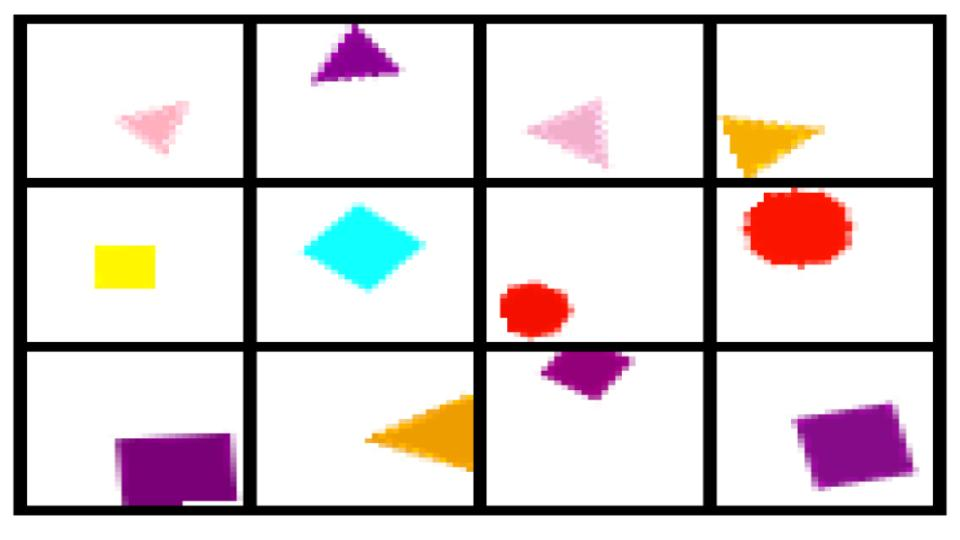
\includegraphics[scale=0.25]{data_sample}
    \caption{An example of synthetic data generated}
    \label{fig:data_sample}
\end{figure}
\subsection{Metrics}
\begin{itemize}
    \item Nearest-neighbor classification on color and shape labels.
    \item Visualization of 2D contrastive embeddings to see if points cluster by color or shape.
    \item Reconstruction Error for the autoencoder
\end{itemize}

\subsection{Results}
\subsubsection{Baseline Approach}
\begin{itemize}
    \item Reconstruction Loss
    \begin{itemize}
        \item $MSE = 0.038 \leftarrow$ lower means better reconstruction
    \end{itemize}
    \item 1-NN Test 
    \begin{itemize}
        \item Color accuracy = 57 \% 
        \item Shape accuracy = 82 \% 
        \item The Bottleneck keeps a strong shape embedding while losing color precision
    \end{itemize}
\end{itemize}

\begin{figure}[h]
    \centering
    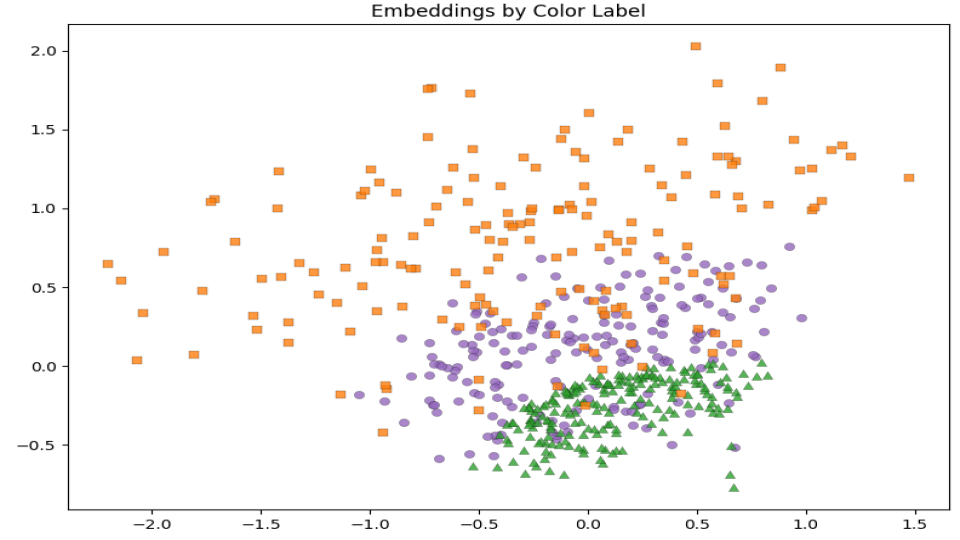
\includegraphics[scale=0.25]{autoencoder_color_label}
    \caption{Autoencoder generated graph for color label}
    \label{fig:autoencoder_color_label1}
\end{figure}
\begin{figure}[h]
    \centering
    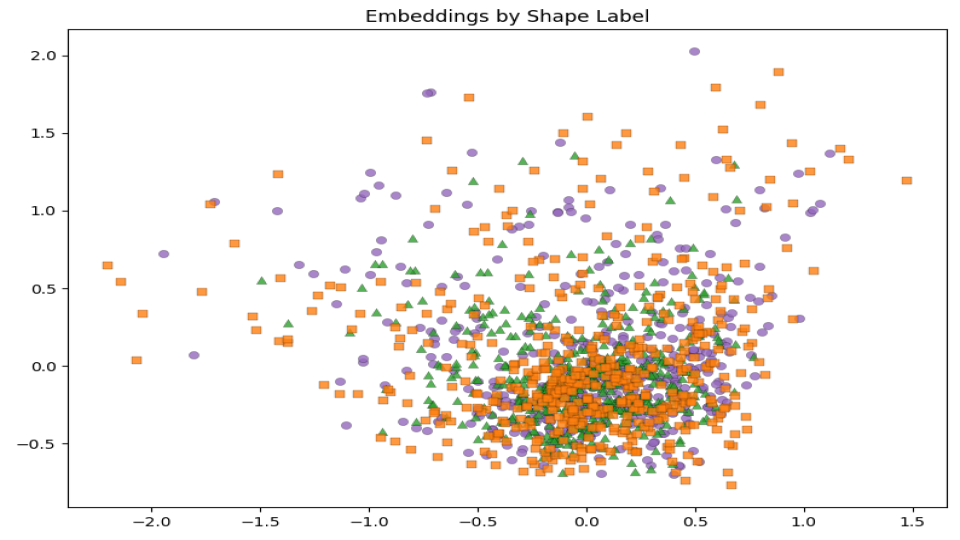
\includegraphics[scale=0.25]{autoencoder_shape_label}
    \caption{Autoencoder generated graph for shape label}
    \label{fig:autoencoder_color_label1}
\end{figure}
\subsubsection{Advanced Approach}
\begin{itemize}
    \item Embeddings don't collapse or explode 
        \begin{itemize}
            \item Allignment $\rightarrow 0.04$, Uniformity $\rightarrow -1.3$
        \end{itemize}
    \item Scatter plots show sectoring for the target attribute
        \begin{itemize}
            \item Color-run: eight color clusters around the circle (shapes random)
            \item Shape-run: three shape clusters around the circle (color random)
        \end{itemize}
    \item 1-NN Test 
        \begin{itemize}
            \item Color-model: color $\approx$ 85\%, shape $\approx$ 33\%
            \item Shape-model: color $\approx$ 35\%, shape $\approx$ 90\%
        \end{itemize}
\end{itemize}
\begin{figure}[h]
    \centering
    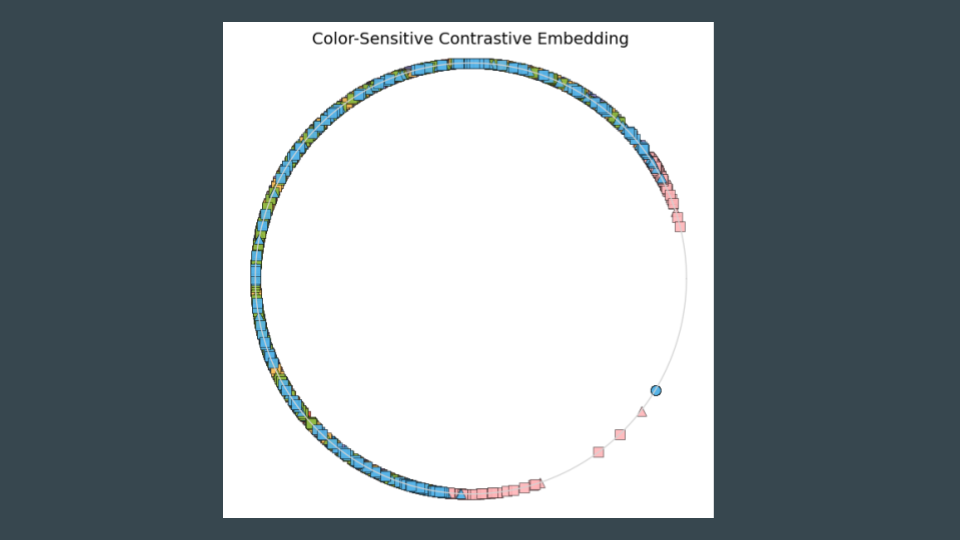
\includegraphics[scale=0.25]{contrastive_color_sensitive}
    \caption{}
    \label{fig:contrastive_color_sensitive1}
\end{figure}
\begin{figure}[h]
    \centering
    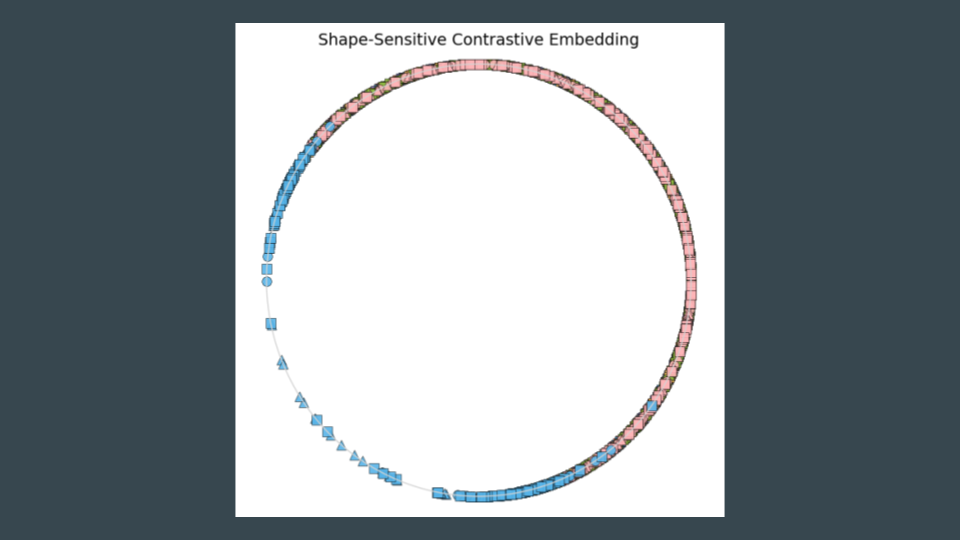
\includegraphics[scale=0.25]{contrastive_shape_sensitive}
    \caption{}
    \label{fig:contrastive_shape_sensitive1}
\end{figure}
\section{Conclusion}
In conclusion our paper replicated two results from \textit{Foundations of Computer Vision}. 
The paper demonstrated the limitation of an autoencoder based approach:
without deeper layer analysis autoencoders will struggle to capture color information.
Furthermore, contrastive models can be used to design what the embedding capture by deploying strategic augmentations.
\subsection{Insights}
The paper illuminates that:
\begin{itemize}
    \item Data augmentation can explicitly bias embeddings to focus on desired features.
    \item Autoencoders, by default, learn reconstructions but do not inherently separate color/shape without deeper layer analysis.
    \item Contrastive learning’s alignment and uniformity objectives reveal an elegant way to impose invariances. 
\end{itemize}
\subsection{Workload}
The project involves:
\begin{itemize}
    \item Implementing data generation scripts.
    \item Implementing the autoencoder and contrastive-learning models in PyTorch.
    \item Running extended experiments (cropping vs. color jitter).
    \item Logging and analyzing results (nearest-neighbor accuracy, 2D embedding plots).
    \item Writing documentation and a final report. 
\end{itemize}
\subsection{Challenges}
Some the key challenges faced in implementing this project were the following.
\begin{itemize}
    \item Learning Pytorch and skLearn
    \item How to contruct a small CNN and autoencoder
    \item How to use 1-NN classifiers to get accuracy scores
    \item Generation of the dataset wasn't entirely trivial and was vital to proper results
\end{itemize}
\section{Duplication Statement}
This project reproduces experiments from \textit{Foundations of Computer Vision}. Online code for the textbook’s examples is not directly used; instead, we will implement everything from scratch. We will ensure our results and code are not merely copies of any existing implementations but a genuine re-implementation and extension (e.g., adjusting resolutions, analyzing color/shape classification). 
\newpage
\section*{References}
\medskip
{
\small
[1] Antonio Torralba, Phillip Isola, \& William T.\ Freeman. (2024). \textit{Foundations of Computer Vision.} The MIT Press. 
}
\end{document}
